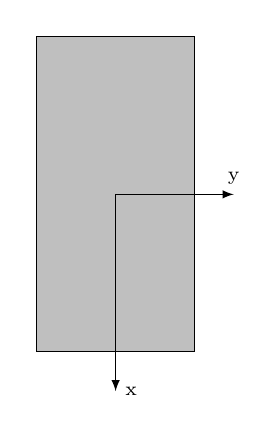
\begin{tikzpicture}
%linee guida
%\foreach \x in {0,1,...,15}
%   \draw [help lines] (\x,0) node [below,%
%          font=\footnotesize] {$\x$} -- (\x,15);
%%\foreach \y in {0,1,...,15}
%%   \draw [help lines] (0,\y) node [left,%
%%          font=\footnotesize] {$\y$} -- (15,\y);

\node at (1,14) (a) {};
\node at (3,14) (b) {};
\node at (3,10) (c) {};
\node at (1,10) (d) {};

\draw[fill=lightgray] (a) rectangle (c);
\draw[-latex] (2,12)--( 2,9.5)node[right]{\scriptsize x};
\draw[-latex] (2,12)--(3.5,12)node[above]{\scriptsize y};


% quote track
 \dimline    [color=gray,
 			  label style={above=0.1ex},
                % line style={thick},
                %extension start style={gray,thin},
                %extension end style={gray,thin},
                extension start length=0.5cm,
                extension end length=0.5cm
                ]{(1,14.5)}{(3,14.5)}{$9$};
                
\dimline    [color=gray,
			label style={above=0.1ex},
                % line style={thick},
                %extension start style={gray,thin},
                %extension end style={gray,thin},
                extension start length=0.5cm,
                extension end length=0.5cm
                ]{(0.5,10)}{(0.5,14)}{$1.5$};
\end{tikzpicture}